% Provenance (never printed): see sources/outline_sources.md (Year 3:
% concordia and discordia; 40Ar/39Ar step heating; Sm-Nd model ages;
% cosmogenic nuclides; fission tracks and (U-Th)/He). Brief:
% sources/book5/BRIEFS.md, ch. 13. Curves from figdata/bachelor-3/
% concordia.py, arar_spectrum.py, model_ages.py, cosmogenic.py. Exercise and
% problem values in the Book 5 scratch calculator calc/ch13.py. The zircons,
% the biotite spectrum, the Nd sample and the helium ages of the Varden
% granite are invented, consistent with the Year 1 volume's granite of 310 Ma.
\chapter{Geokronologi Lanjut}\label{ch:b3:advanced-geochronology}

Sebutir kristal zirkon sepanjang sepersepuluh milimeter telah menjalankan dua jam
sejak granitnya membeku: uranium-238 meluruh menjadi timbal-206 dan
uranium-235 meluruh menjadi timbal-207. Ketika kedua jam itu sepakat, umurnya
tidak lagi diragukan. Jika keduanya berselisih, perselisihan itu sendiri dapat ditanggalkan: kristal
itu kehilangan sebagian timbalnya dalam peristiwa yang lebih muda, dan kedua jam itu, jika dibaca
bersama, memberi umur granit dan umur peristiwa tersebut. Bab ini
membaca beberapa jam sekaligus, dalam uranium dan timbal, dalam argon, dalam neodimium, dalam
jejak fisi dan helium, serta dalam atom langka yang dihasilkan sinar kosmik, dan menjelaskan
seberapa jauh setiap umur dapat dipercaya.

\begin{recall}
Peluruhan radioaktif, persamaan umur, isokron dan rasio awalnya, garis
kuadrat terkecil, peluruhan bercabang, umur kalium--argon, suhu
penutupan dan umur pendinginan ada di volume Tahun 1, dalam bab tentang
penanggalan radiometrik; rumus erosi keadaan tunak \omterm{def:b3:advanced-geochronology:cosmogenic}{nuklida kosmogenik} ada dalam
bab tentang erosi dan transpor. Reservoir seragam kondritik, notasi
epsilon dan mantel terkuras ada di volume Tahun 2, dalam bab tentang
geokimia isotop; ionisasi termal dan spektrometri massa
multikolektor dalam bab tentang metode lapangan dan laboratorium. \omterm{def:b3:orogenic-wedges:thermochronology}{Termokronologi} dan
\omterm{def:b3:orogenic-wedges:age-elevation}{hubungan umur--elevasi} ada dalam \cref{ch:b3:orogenic-wedges}.
\end{recall}

\section{Uranium, timbal, dan konkordia}\label{sec:b3:advanced-geochronology:upb}

Uranium memiliki dua isotop berumur panjang. Uranium-238 meluruh melalui rantai
anak berumur pendek menjadi timbal-206 dengan $\lambda_{238} =
\qty{1.55125e-10}{yr^{-1}}$; uranium-235 meluruh menjadi timbal-207 dengan $\lambda_{235}
= \qty{9.8485e-10}{yr^{-1}}$, enam kali lebih cepat. Rasio kini keduanya ialah
$^{235}\mathrm{U}/^{238}\mathrm{U} = 0.0072567$, atau $^{238}\mathrm{U}/^{235}\mathrm{U}
= 137.8$, sama di setiap batuan terestrial. Zirkon, $\mathrm{ZrSiO_4}$, menyerap
banyak uranium dan hampir tanpa timbal saat terbentuk, serta tahan
terhadap pelapukan dan bertahan dalam metamorfisme: hampir semua timbalnya radiogenik.
% ledger: amherst:constants, tulane:upb-zircon

Tulis $x = {}^{207}\mathrm{Pb}^*/{}^{235}\mathrm{U}$ dan $y =
{}^{206}\mathrm{Pb}^*/{}^{238}\mathrm{U}$ untuk rasio kini timbal radiogenik
terhadap induknya. Masing-masing memberi umur, $t_{206} = \ln(1 + y)/\lambda_{238}$
dan $t_{207} = \ln(1 + x)/\lambda_{235}$.

\begin{definition}[Konkordia, diskordia, titik potong, diagram Tera--Wasserburg]
\label{def:b3:advanced-geochronology:concordia}
Yang disebut \emph{konkordia}\index{konkordia} adalah kurva pada bidang $(x, y)$ tempat
kedua umur uranium--timbal sama. Sebuah \emph{diskordia}\index{diskordia}
adalah garis lurus tempat analisis diskordan dari satu populasi kristal sejajar;
perpotongannya dengan konkordia adalah
\emph{titik potong atas}\index{titik potong atas} (yang lebih tua) dan
\emph{titik potong bawah}\index{titik potong bawah} (yang lebih muda). Sebuah
\emph{diagram Tera--Wasserburg}\index{diagram Tera--Wasserburg} memplot
$X = {}^{238}\mathrm{U}/{}^{206}\mathrm{Pb}^*$ terhadap $Y =
{}^{207}\mathrm{Pb}^*/{}^{206}\mathrm{Pb}^*$.
\end{definition}

\begin{theorem}[Konkordia]\label{thm:b3:advanced-geochronology:concordia}
Sebuah kristal yang tetap tertutup terhadap uranium dan timbal sejak terbentuk,
$t$ yang lalu, terpetakan pada
\[
C(t) = \bigl(e^{\lambda_{235}t} - 1,\; e^{\lambda_{238}t} - 1\bigr).
\]
Ketika $t$ bertambah, kurva naik makin lambat terhadap $x$: kemiringannya,
$\mathrm dy/\mathrm dx = (\lambda_{238}/\lambda_{235})\,e^{(\lambda_{238} -
\lambda_{235})t}$, menurun dari $\lambda_{238}/\lambda_{235} = 0.1575$ di
titik asal, sehingga \omterm{def:b3:advanced-geochronology:concordia}{konkordia} cekung ke arah sumbu $x$.
\end{theorem}

\begin{proof}
Untuk setiap induk, jumlah anak radiogenik per atom induk yang tersisa ialah
$e^{\lambda t} - 1$, persamaan umur dari volume Tahun 1. Mendiferensialkan
kedua koordinat terhadap $t$ lalu membaginya menghasilkan kemiringan; karena
$\lambda_{235} > \lambda_{238}$, kemiringannya menurun seiring $t$.
\end{proof}

Timbal adalah ion besar yang sulit menempati kisi zirkon. Pada bagian kristal
yang rusak oleh radioaktivitasnya sendiri, timbal dapat lepas dalam peristiwa yang
lebih muda berupa pemanasan atau sirkulasi fluida.
% ledger: tulane:upb-zircon

\begin{theorem}[Kehilangan timbal episodik menghasilkan tali busur]\label{thm:b3:advanced-geochronology:discordia}
Sebuah kristal yang terbentuk $t_1$ yang lalu kehilangan, pada $t_2$ yang lalu, pecahan $f$
timbal radiogeniknya dan selebihnya tertutup, terpetakan saat ini pada
\[
(1 - f)\,C(t_1) + f\,C(t_2),
\]
pada tali busur yang menghubungkan titik $t_1$ dan $t_2$ pada \omterm{def:b3:advanced-geochronology:concordia}{konkordia}. Kristal yang
kehilangan pecahan berbeda terletak sepanjang tali busur itu, membentuk \omterm{def:b3:advanced-geochronology:concordia}{diskordia} dengan
\omterm{def:b3:advanced-geochronology:concordia}{titik potong atas} $t_1$ dan \omterm{def:b3:advanced-geochronology:concordia}{titik potong bawah} $t_2$.
\end{theorem}

\begin{proof}
Ambil satu sistem peluruhan dengan konstanta $\lambda$, dan hitung per atom induk
yang ada saat ini. $t_2$ yang lalu terdapat $e^{\lambda t_2}$ atom induk, dan
anak radiogenik $e^{\lambda t_2}(e^{\lambda(t_1 - t_2)} - 1) =
e^{\lambda t_1} - e^{\lambda t_2}$. Peristiwa itu menyisakan $(1 - f)(e^{\lambda t_1} -
e^{\lambda t_2})$; sejak itu induk meluruh lagi sebanyak $e^{\lambda t_2} - 1$. Jumlahnya
adalah $(1 - f)(e^{\lambda t_1} - 1) + f(e^{\lambda t_2} - 1)$. Kedua isotop timbal
berperilaku serupa secara kimia, sehingga $f$ sama untuk keduanya, dan kedua koordinat
bergabung menjadi titik yang dinyatakan.
\end{proof}

\begin{omfigure}
\begin{tikzpicture}
\begin{groupplot}[group style={group size=2 by 1, horizontal sep=1.7cm},
  omrecord, width=0.47\linewidth, height=0.42\linewidth, title style={font=\small},
  tick label style={font=\scriptsize}, label style={font=\small}]
\nextgroupplot[title={(a) diagram konkordia},
  xlabel={$^{207}\mathrm{Pb}^*/^{235}\mathrm{U}$}, ylabel={$^{206}\mathrm{Pb}^*/^{238}\mathrm{U}$},
  xmin=0.04, xmax=0.44, ymin=0.006, ymax=0.06,
  xtick={0.1,0.2,0.3,0.4}, xticklabels={0.1,0.2,0.3,0.4},
  ytick={0.01,0.02,0.03,0.04,0.05}, yticklabels={0.01,0.02,0.03,0.04,0.05},
  scaled ticks=false]
% computed in figdata/bachelor-3/concordia.py
\addplot[black, thick] table[x=xw, y=yw] {figdata/out/bachelor-3-concordia-curve.dat};
\addplot[black, only marks, mark=*, mark size=1.4pt, nodes near coords={\scriptsize\pgfmathprintnumber[fixed, precision=0]{\pgfplotspointmeta}},
  point meta=explicit, nodes near coords align={anchor=south east},
  restrict expr to domain={\thisrow{t}}{100:350}]
  table[x=xw, y=yw, meta=t] {figdata/out/bachelor-3-concordia-ticks.dat};
\addplot[omDef, thick, densely dashed] table[x=x, y=y] {figdata/out/bachelor-3-concordia-line.dat};
\addplot[red!70!black, only marks, mark=diamond*, mark size=2pt] table[x=x, y=y] {figdata/out/bachelor-3-concordia-zircons.dat};
\nextgroupplot[title={(b) diagram Tera--Wasserburg},
  xlabel={$^{238}\mathrm{U}/^{206}\mathrm{Pb}^*$}, ylabel={$^{207}\mathrm{Pb}^*/^{206}\mathrm{Pb}^*$},
  xmin=15, xmax=75, ymin=0.0465, ymax=0.0535,
  ytick={0.047,0.049,0.051,0.053}, yticklabels={0.047,0.049,0.051,0.053},
  scaled ticks=false]
\addplot[black, thick] table[x=xtw, y=ytw] {figdata/out/bachelor-3-concordia-curve.dat};
\addplot[black, only marks, mark=*, mark size=1.4pt, nodes near coords={\scriptsize\pgfmathprintnumber[fixed, precision=0]{\pgfplotspointmeta}},
  point meta=explicit, nodes near coords align={anchor=north east},
  restrict expr to domain={\thisrow{t}}{100:250}]
  table[x=xtw, y=ytw, meta=t] {figdata/out/bachelor-3-concordia-ticks.dat};
\addplot[omDef, thick, densely dashed] table[x=xtw, y=ytw] {figdata/out/bachelor-3-concordia-twline.dat};
\addplot[red!70!black, only marks, mark=diamond*, mark size=2pt] table[x=xtw, y=ytw] {figdata/out/bachelor-3-concordia-zircons.dat};
\end{groupplot}
\end{tikzpicture}

\par\smallskip{\small (a) \omterm{def:b3:advanced-geochronology:concordia}{Konkordia}, dengan umurnya dalam jutaan tahun,
dan lima zirkon diskordan rekaan dari satu granit (merah; elips galatnya
lebih kecil daripada simbolnya), berjajar pada \omterm{def:b3:advanced-geochronology:concordia}{diskordia} (putus-putus) yang
memotong \omterm{def:b3:advanced-geochronology:concordia}{konkordia} di dekat 311 dan \qty{100}{\Ma}. (b) Zirkon dan garis yang sama
dalam \omterm{def:b3:advanced-geochronology:concordia}{diagram Tera--Wasserburg}, tempat \omterm{def:b3:advanced-geochronology:concordia}{diskordia} tetap berupa garis
lurus.}\label{fig:b3:advanced-geochronology:concordia}
\end{omfigure}
% ledger: amherst:constants

Titik potong diperoleh dari kondisi $a + b\,x(t) = y(t)$, persamaan dalam $t$ yang
diselesaikan dengan metode Newton. Misalkan $g(t) = e^{\lambda_{238}t} - 1 - a -
b(e^{\lambda_{235}t} - 1)$ dan $g'(t) = \lambda_{238}e^{\lambda_{238}t} -
b\lambda_{235}e^{\lambda_{235}t}$, iterasikan $t \leftarrow t - g/g'$ dari tebakan
di dekat setiap titik potong. Tiga sifat hasil ini penting dalam praktik.
Pertama, \omterm{def:b3:advanced-geochronology:concordia}{titik potong atas} hanya presisi jika \omterm{def:b3:advanced-geochronology:concordia}{diskordia} memotong
\omterm{def:b3:advanced-geochronology:concordia}{konkordia} pada sudut besar. \omterm{def:b3:advanced-geochronology:concordia}{Diskordia} muda, seperti pada gambar di atas, berjalan
hampir sepanjang \omterm{def:b3:advanced-geochronology:concordia}{konkordia}, dan perubahan kecil pada kemiringannya menggeser
titik potong jauh. Kedua, jika kehilangan timbal baru-baru ini, $t_2 = 0$, \omterm{def:b3:advanced-geochronology:concordia}{diskordia}
melalui titik asal, dan setiap kristal memiliki
rasio $^{207}\mathrm{Pb}^*/^{206}\mathrm{Pb}^*$ yang sama,
\[
\frac{^{207}\mathrm{Pb}^*}{^{206}\mathrm{Pb}^*} = \frac{1}{137.8}\,
\frac{e^{\lambda_{235}t_1} - 1}{e^{\lambda_{238}t_1} - 1},
\]
yang memberikan $t_1$ tanpa uranium: umur timbal--timbal. Ketiga, garis dalam
diagram \omterm{def:b3:advanced-geochronology:concordia}{konkordia}, $x = (y - a)/b$, menjadi dalam koordinat Tera--Wasserburg
$Y = (1 - aX)/(137.8\,b)$, kembali berupa garis. \omterm{def:b3:advanced-geochronology:concordia}{Diagram Tera--Wasserburg}
menggunakan rasio yang diukur langsung, tanpa perlu menghitung uranium-235
dari uranium-238, dan campuran dengan timbal biasa, tidak radiogenik dan kaya
timbal-207, terletak pada garis yang mencapai sumbu $Y$ pada rasio timbal
biasa.

Umur uranium--timbal diukur dengan dua cara. Kristal tunggal atau fragmen,
dilarutkan setelah zona rusak dihilangkan dengan pelarutan parsial
dan timbal serta uranium mereka dipisahkan, diukur dengan spektrometri massa ionisasi termal
dengan umur paling presisi dalam geologi. Titik analisis selebar beberapa puluh
mikrometer diukur langsung di tempat, dengan probe ion atau dengan
ablasi laser, kurang presisi tetapi zona demi zona melalui kristal yang tumbuh dalam
beberapa peristiwa.

\begin{inthelab}[Laboratorium geokronologi]
\begin{minipage}[t]{0.55\linewidth}\vspace{0pt}
Penanggalan zirkon dimulai dari batuan yang dihancurkan dan berakhir di laboratorium bersih. Para
ahli geokronologi memisahkan zirkon berdasarkan massa jenis dan kemagnetan, lalu memilih
kristal yang paling jernih di bawah mikroskop binokular dan mencitrakan zonasinya. Kristal
dilarutkan sebagian untuk menghilangkan zona rusaknya, lalu dilarutkan seluruhnya dengan
spike isotop yang diketahui, dan uranium serta timbal dipisahkan
pada kolom resin yang sangat kecil, di udara yang disaring untuk menahan timbal dari
debu. Spektrometer massa mengukur rasio isotop. Sampel argon mengikuti
jalur yang berbeda: reaktor, lalu jalur gas tempat laser memanaskan setiap tahap dan
argon dibersihkan sebelum masuk ke spektrometer.
\end{minipage}\hfill
\begin{minipage}[t]{0.42\linewidth}\vspace{0pt}
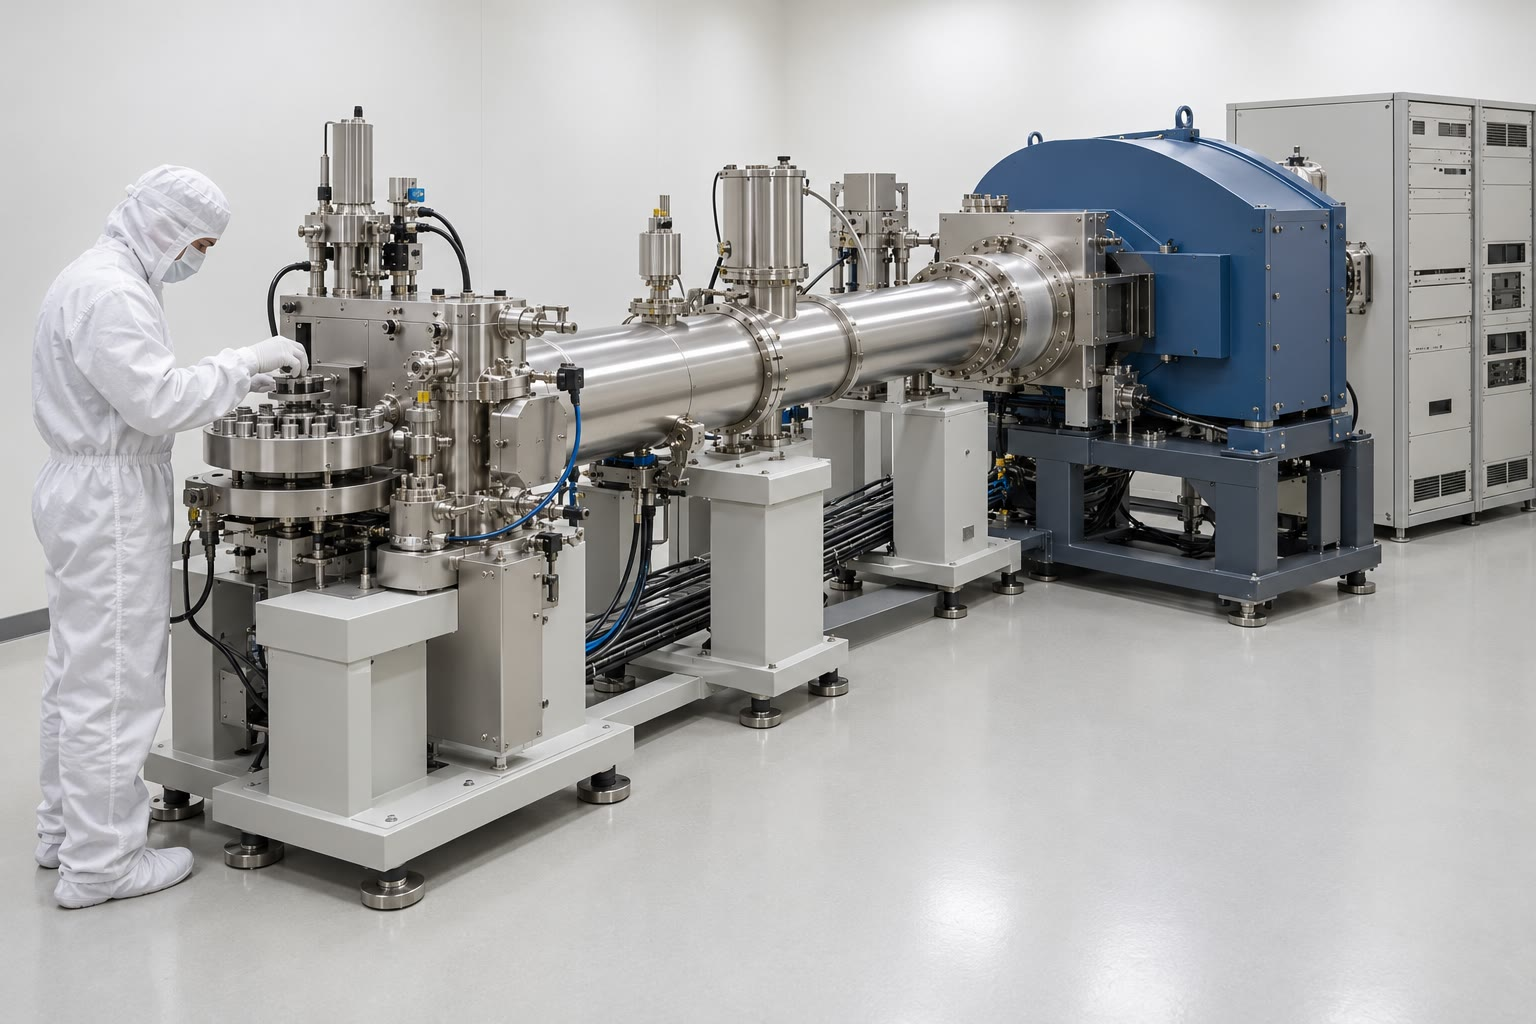
\includegraphics[width=\linewidth]{images/book5/ai/b3-mass-spec-lab.jpg}

{\scriptsize Spektrometer massa di laboratorium bersih: turet sampel di
kiri, tabung terbang dan elektromagnet (ilustrasi buatan
AI).}
\end{minipage}
\end{inthelab}

\section{Penanggalan argon--argon}\label{sec:b3:advanced-geochronology:arar}

Metode kalium--argon pada volume Tahun 1 mengukur kalium dan
argon dalam dua aliquot terpisah dari sebuah mineral. Metode argon--argon
hanya mengukur argon, dalam satu aliquot, sebagai rasio isotop. Sampel
diiradiasi dengan neutron cepat di inti reaktor nuklir, tempat
reaksi $^{39}\mathrm{K}(n,p)^{39}\mathrm{Ar}$ mengubah sebagian tetap dari
kalium-39-nya menjadi argon-39, sebagai proksi kalium. Sebuah mineral berumur diketahui, yakni
monitor, diiradiasi di sebelahnya.
% ledger: nmgrl:arar, amherst:arar

\begin{definition}[Penanggalan argon--argon, faktor J, spektrum umur, umur plato]
\label{def:b3:advanced-geochronology:arar}
\emph{Penanggalan $^{40}\mathrm{Ar}/^{39}\mathrm{Ar}$}\index{penanggalan argon--argon@penanggalan $^{40}\mathrm{Ar}/^{39}\mathrm{Ar}$}
menentukan umur mineral yang mengandung kalium melalui rasio $R =
{}^{40}\mathrm{Ar}^*/{}^{39}\mathrm{Ar}_{\mathrm K}$ dari argon-40 radiogeniknya
ke argon-39 yang dibentuk dari kaliumnya melalui iradiasi neutron. Yang disebut
\emph{faktor J}\index{faktor J} dari suatu iradiasi adalah $J = (e^{\lambda
t_m} - 1)/R_m$, diperoleh dari monitor berumur diketahui $t_m$ dan rasio terukur
$R_m$, dengan $\lambda$ konstanta peluruhan total kalium-40. Ketika sampel
dikeluarkan gasnya secara bertahap pada suhu yang meningkat, \emph{spektrum
umur}\index{spektrum umur} menampilkan umur tiap tahap terhadap
fraksi kumulatif argon-39 yang dilepaskan. Yang disebut \emph{umur
plato}\index{umur plato} adalah rata-rata terbobot umur tahap-tahap berurutan yang
sepakat dalam batas ketidakpastiannya dan melepaskan sebagian besar argon-39.
\end{definition}

\begin{theorem}[Umur argon--argon]\label{thm:b3:advanced-geochronology:arar}
Sampel yang diiradiasi bersama monitor memiliki umur
\[
t = \frac1\lambda\ln(1 + JR).
\]
\end{theorem}

\begin{proof}
Argon radiogenik adalah $^{40}\mathrm{Ar}^* = (\lambda_e/\lambda)\,
{}^{40}\mathrm{K}\,(e^{\lambda t} - 1)$, menurut peluruhan bercabang pada
volume Tahun 1. Argon-39 yang terbentuk adalah $^{39}\mathrm{Ar}_{\mathrm K} =
{}^{39}\mathrm{K}\,\Phi$, dengan $\Phi$ menghimpun dosis neutron dan
penampang lintang reaksi. Dengan demikian $R = (e^{\lambda t} - 1)/J$ dengan $J =
\lambda\,\Phi\,{}^{39}\mathrm{K}/(\lambda_e\,{}^{40}\mathrm{K})$. Rasio
$^{40}\mathrm{K}/^{39}\mathrm{K}$ sama di semua kalium, dan $\Phi$
sama untuk dua sampel yang diiradiasi berdampingan, sehingga $J$ sama untuk sampel
dan monitor; umur dan rasio monitor memberikannya, dan membalik $R$ memberikan
$t$.
\end{proof}

Konstanta yang dipakai adalah milik metode kalium--argon, $\lambda =
\qty{5.543e-10}{yr^{-1}}$. Monitor yang umum adalah sanidin dari tuf vulkanik
berumur \qty{28.201}{\Ma}; rasio monitor $R_m = 1.3129$ memberikan $J =
0.01200$. Argon atmosfer, dengan $^{40}\mathrm{Ar}/^{36}\mathrm{Ar} = 295.5$,
dikurangkan dengan argon-36 yang diukur pada setiap tahap, dan argon yang dibentuk oleh
neutron dari kalsium dan dari kalium itu sendiri dikoreksi dengan garam
yang diiradiasi dalam kemasan yang sama.
% ledger: schaen20:monitors, amherst:constants, nmgrl:arar

Pemanasan bertahap merupakan kekuatan metode ini. Sampel dipanaskan dalam tungku
atau dengan laser dalam tahap-tahap suhu yang makin naik, dan setiap tahap menghasilkan satu umur.
Jika mineral tetap tertutup sejak mendingin, semua tahap sepakat: spektrumnya
datar. Jika mineral kehilangan argon dari tepi butirnya, tahap-tahap awal, yang
berasal dari tepi, lebih muda, dan umurnya naik bertangga menuju sebuah
plato yang ditentukan oleh inti butir. Kriteria yang dianjurkan untuk sebuah plato adalah
setidaknya lima tahap berurutan yang memuat lebih dari \qty{50}{\percent} argon-39,
tanpa tren di antaranya; tahap suhu rendah pada spektrum bertangga biasanya dibaca sebagai
kehilangan argon radiogenik. Argon berlebih, yang terperangkap dari suatu fluida saat mineral
tumbuh, berefek sebaliknya: ia membuat beberapa tahap menjadi terlalu tua, yang sering berupa tahap pertama
dan terakhir, dalam spektrum berbentuk pelana. Jumlah semua tahap, yakni umur total-gas, adalah
yang akan diberikan oleh umur kalium--argon: sebuah rata-rata
yang menyembunyikan riwayatnya.
% ledger: schaen20:plateau, nmgrl:arar

\begin{omfigure}
\begin{tikzpicture}
\begin{groupplot}[group style={group size=2 by 1, horizontal sep=1.5cm},
  omrecord, height=0.38\linewidth, title style={font=\small},
  xlabel={kumulatif $^{39}\mathrm{Ar}$ yang terlepas (\unit{\percent})},
  tick label style={font=\scriptsize}, label style={font=\small}]
\nextgroupplot[title={(a) seluruh spektrum}, width=0.52\linewidth,
  ylabel={umur semu (\unit{\Ma})}, xmin=0, xmax=100, ymin=130, ymax=320,
  xtick={0,20,40,60,80,100}, ytick={150,200,250,300}]
% computed in figdata/bachelor-3/arar_spectrum.py
\addplot[omDef, thick] table[x=cum, y=age] {figdata/out/bachelor-3-arar_spectrum-boxes.dat};
\node[font=\scriptsize, anchor=west] at (axis cs:12,180) {kehilangan argon};
\node[font=\scriptsize, anchor=north, red!70!black] at (axis cs:59,290) {plato};
\nextgroupplot[title={(b) plato, diperbesar}, width=0.44\linewidth,
  xmin=15, xmax=100, ymin=290, ymax=300, xtick={20,40,60,80,100},
  ytick={290,292,294,296,298,300}]
\addplot[name path=hi, draw=none, forget plot] table[x=cum, y=hi] {figdata/out/bachelor-3-arar_spectrum-boxes.dat};
\addplot[name path=lo, draw=none, forget plot] table[x=cum, y=lo] {figdata/out/bachelor-3-arar_spectrum-boxes.dat};
\addplot[omDef!25, forget plot] fill between[of=hi and lo];
\addplot[omDef, thick] table[x=cum, y=age] {figdata/out/bachelor-3-arar_spectrum-boxes.dat};
\draw[red!70!black, thick] (axis cs:18,296.1) -- (axis cs:100,296.1);
\node[font=\scriptsize, anchor=south, red!70!black] at (axis cs:59,290.3) {plato \qty[separate-uncertainty=true]{296.1 \pm 0.8}{\Ma}};
\end{groupplot}
\end{tikzpicture}

\par\smallskip{\small \omterm{def:b3:advanced-geochronology:arar}{Spektrum umur} rekaan untuk biotit dari granit pada
gambar pertama: setiap tahap digambar pada umurnya, lebarnya menunjukkan bagian
argon-39 yang dilepaskannya. (a) Tiga tahap suhu rendah naik bertangga menuju sebuah
plato. (b) Ketujuh tahap plato, yang memuat \qty{82}{\percent} dari
argon-39, dengan rentang dua simpangan baku (diarsir) dan \omterm{def:b3:advanced-geochronology:arar}{umur plato}
(merah).}\label{fig:b3:advanced-geochronology:spectrum}
\end{omfigure}

\section{Umur model neodimium}\label{sec:b3:advanced-geochronology:model-age}

Ketika lelehan diekstraksi dari mantel untuk membentuk kerak benua, samarium,
yang lebih kompatibel, tertinggal lebih banyak daripada neodimium: kerak baru memiliki
$^{147}\mathrm{Sm}/^{144}\mathrm{Nd}$ yang lebih rendah daripada sumbernya, sekitar 0.13 untuk sebagian besar
batuan kerak, dibandingkan dengan 0.1966 untuk reservoir kondritik. Rasio
$^{143}\mathrm{Nd}/^{144}\mathrm{Nd}$ kemudian tumbuh lebih lambat.
Setelah terbentuk, batuan kerak cenderung mempertahankan rasio samarium--neodimiumnya,
melalui erosi, sedimentasi, dan bahkan peleburan ulang, sehingga neodimiumnya mengingat kapan ia meninggalkan
mantel.
% ledger: white08:model-age, white:chur

\begin{definition}[Umur model]\label{def:b3:advanced-geochronology:model-age}
Yang disebut \emph{umur model}\index{umur model} suatu batuan dalam sistem isotop adalah
waktu saat rasionya, diproyeksi mundur dengan rasio induk--anak masa kininya,
sama dengan rasio suatu reservoir model. Untuk neodimium, $T_{\mathrm{CHUR}}$
menggunakan reservoir seragam kondritik, dan $T_{\mathrm{DM}}$ memakai mantel
terkuras.
\end{definition}

\begin{theorem}[Umur model]\label{thm:b3:advanced-geochronology:model-age}
Sampel dengan rasio masa kini $I_s = {}^{143}\mathrm{Nd}/^{144}\mathrm{Nd}$ dan
$R_s = {}^{147}\mathrm{Sm}/^{144}\mathrm{Nd}$, dibandingkan dengan reservoir yang
rasio masa kininya $I_m$ dan $R_m$, memiliki \omterm{def:b3:advanced-geochronology:model-age}{umur model}
\[
T = \frac1\lambda\ln\left(1 + \frac{I_s - I_m}{R_s - R_m}\right),
\qquad \lambda = \lambda_{147}.
\]
\end{theorem}

\begin{proof}
Sistem tertutup, $T$ waktu lalu, memiliki rasio $I - R(e^{\lambda T} - 1)$: persamaan
isokron dibaca mundur. Dengan menyamakan ini untuk sampel dan
reservoir menghasilkan $I_s - I_m = (R_s - R_m)(e^{\lambda T} - 1)$.
\end{proof}

Dengan $\lambda_{147} = \qty{6.524e-12}{yr^{-1}}$, reservoir yang dipakai adalah
yang kondritik, dengan 0.512638 dan 0.1966 pada masa kini, dan mantel terkuras,
0.51315 pada masa kini, sekitar $\varepsilon_{\mathrm{Nd}} = +10$, yang diperoleh
oleh evolusi tertutup dari nilai kondritik sejak \qty{4.55}{\Ga} lalu, dengan rasio
$^{147}\mathrm{Sm}/^{144}\mathrm{Nd} = 0.2137$. Sebuah granit rekaan dengan
$I_s = 0.511900$ dan $R_s = 0.1100$ memiliki $\varepsilon_{\mathrm{Nd}} = -14.4$
pada masa kini, $T_{\mathrm{CHUR}} = \qty{1.30}{\Ga}$ dan $T_{\mathrm{DM}} =
\qty{1.84}{\Ga}$. Gambar di bawah membaca keduanya. Umur mantel terkuras adalah
taksiran yang lebih baik, karena kerak diekstraksi dari mantel yang sudah
terkuras; ia adalah umur rata-rata saat neodimium sampel meninggalkan
mantel, yaitu umur tinggal kerak. Dua peringatan membatasinya: kerak tidak boleh
telah mengubah rasio samarium--neodimiumnya sejak itu, dan batuan yang terbentuk dari pencampuran
kerak tua dengan lelehan mantel baru memiliki \omterm{def:b3:advanced-geochronology:model-age}{umur model} antara yang tidak bermakna.
% ledger: villa20:sm147, white:chur, white08:model-age

\begin{omfigure}
\begin{tikzpicture}
\begin{axis}[omrecord, width=0.72\linewidth, height=0.38\linewidth,
  xlabel={waktu sebelum masa kini (\unit{\Ga})}, ylabel={$\varepsilon_{\mathrm{Nd}}$},
  xmin=0, xmax=2.5, ymin=-17, ymax=13, x dir=reverse,
  xtick={0,0.5,1,1.5,2,2.5}, xticklabels={0,0.5,1,1.5,2,2.5},
  tick label style={font=\scriptsize}, label style={font=\small},
  legend style={font=\scriptsize, at={(0.5,1.03)}, anchor=south, legend columns=3, legend cell align=left}]
% computed in figdata/bachelor-3/model_ages.py
\addplot[omDef, thick] table[x=t, y=eps_dm] {figdata/out/bachelor-3-model_ages-evolution.dat};
\addlegendentry{mantel terkuras}
\addplot[black, thick, densely dashed] coordinates {(0,0) (2.5,0)};
\addlegendentry{CHUR}
\addplot[red!70!black, thick] table[x=t, y=eps_sample] {figdata/out/bachelor-3-model_ages-evolution.dat};
\addlegendentry{granit}
\draw[densely dotted] (axis cs:1.30,0) -- (axis cs:1.30,-17) node[above right, font=\scriptsize, rotate=90] {$T_{\mathrm{CHUR}}$};
\draw[densely dotted] (axis cs:1.84,5.4) -- (axis cs:1.84,-17) node[above right, font=\scriptsize, rotate=90] {$T_{\mathrm{DM}}$};
\end{axis}
\end{tikzpicture}

\par\smallskip{\small $\varepsilon_{\mathrm{Nd}}$ dari granit rekaan yang diproyeksikan
mundur dalam waktu dengan rasio samarium--neodimium miliknya sendiri (merah). Kurva ini memotong
reservoir seragam kondritik pada $T_{\mathrm{CHUR}} = \qty{1.30}{\Ga}$ dan mantel
terkuras (biru) pada $T_{\mathrm{DM}} = \qty{1.84}{\Ga}$.}\label{fig:b3:advanced-geochronology:model-age}
\end{omfigure}

\section{Jejak fisi dan helium}\label{sec:b3:advanced-geochronology:low-t}

Uranium-238 juga meluruh, sangat jarang, melalui fisi spontan: inti
terbelah menjadi dua fragmen yang terpental berpisah dan meninggalkan jejak kerusakan dalam
kristal, selebar hingga \qty{9}{nm} dan sepanjang sekitar \qty{23}{\micro\metre} pada
apatit. Setelah dietsa dengan asam, jejak itu tampak di bawah mikroskop.
Jejak itu pulih ketika kristal dipanaskan, pada rentang sekitar 20 hingga \qty{350}{\celsius}
bergantung pada mineralnya; pada apatit, jejak itu memendek di dalam
zona penganilan parsial, sekitar 60 hingga \qty{120}{\celsius}, dan lenyap di atasnya.
% ledger: kohn24:ft, sueoka19:closure

\begin{definition}[Penanggalan jejak fisi, penganilan jejak]\label{def:b3:advanced-geochronology:fission-track}
Yang disebut \emph{penanggalan jejak fisi}\index{penanggalan jejak fisi} menentukan umur mineral
berdasarkan massa jenis jejak yang ditinggalkan di dalamnya oleh fisi spontan
uranium-238, dibandingkan dengan kandungan uraniumnya. Yang disebut \emph{penganilan
jejak}\index{penganilan jejak} adalah pemendekan dan hilangnya
jejak akibat perbaikan kristal saat dipanaskan.
\end{definition}

\begin{theorem}[Umur jejak fisi]\label{thm:b3:advanced-geochronology:fission-track}
Dengan $\lambda_f$ konstanta peluruhan fisi spontan dan $\lambda =
\lambda_{238}$ konstanta total, sebuah kristal dengan $N_s$ fisi spontan per satuan
volume dan $N$ atom uranium-238 memiliki umur
\[
t = \frac1\lambda\ln\left(1 + \frac{\lambda}{\lambda_f}\,\frac{N_s}{N}\right).
\]
Di laboratorium, uranium diukur dengan menginduksi fisi
uranium-235 dengan neutron termal, dan umur menjadi
\[
t = \frac1\lambda\ln\left(1 + \lambda\,\zeta\,g\,\rho_d\,\frac{\rho_s}{\rho_i}\right),
\]
dengan $\rho_s$ dan $\rho_i$ massa jenis jejak spontan dan terinduksi,
$\rho_d$ massa jenis jejak pada kaca dosimeter, $g = 0.5$ faktor geometri
dan $\zeta$ konstanta kalibrasi yang diperoleh dari standar dengan umur yang diketahui.
\end{theorem}

\begin{proof}
Uranium-238 telah meluruh sebanyak $N(e^{\lambda t} - 1)$ kali, dan fraksi
$\lambda_f/\lambda$ dari peluruhan ini adalah fisi: $N_s =
(\lambda_f/\lambda)N(e^{\lambda t} - 1)$, yang dapat disusun ulang menjadi bentuk pertama.
Massa jenis jejak sebanding dengan $N_s$ dan dengan jumlah
fisi terinduksi, $N\,\sigma\,\Phi/137.8$, dengan $\sigma$ adalah penampang lintang fisi
uranium-235 dan $\Phi$ fluensi neutron, yang sendirinya
sebanding dengan $\rho_d$. Rasio $\rho_s/\rho_i$ kemudian sama dengan $N_s/N$ dikalikan
hasil kali sejumlah konstanta, dan $\lambda_f$, $\sigma$, $137.8$ serta efisiensi
pengetsaan dan penghitungan digabungkan bersama $g$ ke dalam $\zeta$.
\end{proof}

Konstanta peluruhan fisi hanya diketahui hingga sekitar \qty{10}{\percent},
antara \num{7.9e-17} dan \qty{8.7e-17}{yr^{-1}}, itulah sebabnya sebagian besar
laboratorium lebih memilih kalibrasi $\zeta$. Panjang jejak menyimpan
catatan lintasan suhu. Batuan yang mendingin cepat melewati
zona penganilan parsial memiliki jejak panjang dengan panjang hampir sama; batuan yang
tertahan di dalamnya memiliki jejak lebih pendek dengan panjang yang tersebar luas, dan
umur jejak fisi lalu menjadi umur campuran, bukan waktu saat melewati satu
suhu.
% ledger: kohn24:ft

\begin{omfigure}
\begin{tikzpicture}[scale=0.85]
% (a) an etched apatite grain with tracks
\draw[thick, fill=omLithLime!15] (0,0) -- (3.2,0) -- (3.8,1.0) -- (3.2,2.0) -- (0,2.0) -- (-0.6,1.0) -- cycle;
\foreach \x/\y/\a in {0.4/0.5/30, 1.2/1.3/-20, 2.0/0.6/75, 2.6/1.4/10, 0.9/1.6/110, 1.7/0.9/150, 2.9/0.8/50}
  {\draw[very thick, black] (\x,\y) -- ++(\a:0.45);}
\node[font=\small] at (1.6,-0.4) {(a) jejak hasil etsa pada apatit};
% (b) alpha ejection from a grain
\begin{scope}[xshift=6cm]
\draw[thick, fill=omLithLime!15] (0,0) rectangle (3.4,2.0);
\draw[dashed] (0.35,0.35) rectangle (3.05,1.65);
\fill[black] (0.2,1.0) circle (1.5pt) node[below right, font=\scriptsize] {U};
\draw[->, red!70!black, thick] (0.2,1.0) -- ++(160:0.7) node[left, font=\scriptsize] {He hilang};
\fill[black] (1.7,1.0) circle (1.5pt);
\draw[->, red!70!black, thick] (1.7,1.0) -- ++(40:0.5);
\node[font=\scriptsize, align=center] at (1.7,0.55) {He tertahan};
\draw[<->] (3.05,1.8) -- (3.4,1.8) node[right, font=\scriptsize] {\qty{20}{\micro\metre}};
\node[font=\small] at (1.7,-0.4) {(b) pelepasan alfa};
\end{scope}
\end{tikzpicture}

\par\smallskip{\small Skema. (a) Jejak fisi spontan, yang diungkap dengan
pengetsaan pada butir apatit yang dipoles, dihitung per satuan luas. (b) Partikel alfa
menempuh sekitar \qty{20}{\micro\metre}: yang dipancarkan dalam jarak tersebut
dari permukaan (di luar garis putus-putus) mungkin keluar dari butir, sehingga
butir kecil menyimpan lebih sedikit heliumnya.}\label{fig:b3:advanced-geochronology:low-t}
\end{omfigure}
% ledger: zeigler23:ejection

Setiap peluruhan alfa memancarkan inti helium-4. Uranium, torium, dan rantai peluruhannya
menumpuk helium di dalam kristal, yang hanya menyimpannya saat dingin.

\begin{definition}[Penanggalan (U--Th)/He, zona retensi parsial]\label{def:b3:advanced-geochronology:uthhe}
Yang disebut \emph{penanggalan (U--Th)/He}\index{penanggalan U--Th/He@penanggalan (U--Th)/He} menentukan umur
mineral berdasarkan helium-4 yang terakumulasi dari peluruhan alfa uranium, torium
dan anak radiogeniknya, dibandingkan dengan kandungan uranium dan toriumnya. Yang disebut \emph{zona
retensi parsial}\index{zona retensi parsial} adalah rentang suhu tempat
helium yang terbentuk sebagian tertahan dan sebagian hilang akibat difusi.
\end{definition}

\begin{theorem}[Pertumbuhan helium]\label{thm:b3:advanced-geochronology:helium}
Sebuah kristal yang tertutup bagi helium selama waktu $t$ memuat
\[
\mathrm{He} = 8\,{}^{238}\mathrm U\,(e^{\lambda_{238}t} - 1)
+ 7\,{}^{235}\mathrm U\,(e^{\lambda_{235}t} - 1)
+ 6\,{}^{232}\mathrm{Th}\,(e^{\lambda_{232}t} - 1),
\]
dalam atom, dengan induk diukur saat ini; samarium-147 menambahkan suku kecil.
\end{theorem}

\begin{proof}
Setiap rantai kehilangan selisih massanya dalam partikel alfa, masing-masing empat satuan massa:
$(238 - 206)/4 = 8$, $(235 - 207)/4 = 7$, $(232 - 208)/4 = 6$, sedangkan peluruhan
beta tidak mengubah nomor massa. Setiap rantai berada dalam kesetimbangan sekuler,
sehingga setiap peluruhan induk diikuti oleh seluruh rantainya, dan jumlah
peluruhan tiap induk sama dengan yang ada di persamaan umur.
\end{proof}

Untuk kristal muda, $e^{\lambda t} - 1 \approx \lambda t$ dan umurnya diperoleh
dari satu kali pembagian. Partikel alfa menempuh sekitar
\qty{20}{\micro\metre} sebelum berhenti, sehingga kristal kehilangan helium yang terbentuk
dekat permukaannya; umur terukur dibagi dengan fraksi tertahan $F_T$,
yang lebih kecil untuk butir kecil ($F_T = 0.70$ berarti \qty{30}{\percent}
hilang). Apatit menutup terhadap helium pada sekitar 50 sampai \qty{80}{\celsius}, zirkon pada
160 sampai \qty{200}{\celsius}: dengan jejak fisi apatit, sekitar 90 sampai
\qty{120}{\celsius}, kronometer suhu rendah menanggalkan
beberapa kilometer terakhir naiknya batuan ke permukaan, sebagaimana
dipakai pada \cref{ch:b3:orogenic-wedges}.
% ledger: zeigler23:ejection, sueoka19:closure, iaea:isotopes

\section{Nuklida kosmogenik}\label{sec:b3:advanced-geochronology:cosmogenic}

Sinar kosmik yang menghantam atmosfer membentuk hujan partikel sekunder. Neutron
cepat yang mencapai permukaan memecah inti atom dalam mineral pada
beberapa meter teratas batuan, melalui spalasi: oksigen dalam kuarsa menjadi berilium-10, silikon
menjadi aluminium-26. Muon membentuk sebagian nuklida lebih dalam dan mendominasi di bawah
sekitar \qty{3}{m}.
% ledger: zech04:exposure, portenga:method

\begin{definition}[Nuklida kosmogenik, umur keterpaparan, laju produksi]
\label{def:b3:advanced-geochronology:cosmogenic}
Yang disebut \emph{nuklida kosmogenik}\index{nuklida kosmogenik} ialah
nuklida yang terbentuk dalam mineral di atau dekat permukaan oleh partikel sekunder sinar kosmik. Laju
\emph{laju produksi}\index{laju produksi (kosmogenik)} $P$ adalah jumlah
atom yang terbentuk per satuan massa mineral dan per tahun. \emph{Umur
keterpaparan}\index{umur keterpaparan} suatu permukaan adalah waktu sejak pertama kali terpapar
ke sinar kosmik, dihitung dari konsentrasi nuklida kosmogenik.
\end{definition}

\omterm{def:b3:advanced-geochronology:cosmogenic}{Laju produksi} berkurang terhadap kedalaman sebagai $P_0e^{-\rho z/\Lambda}$, dengan
panjang atenuasi diambil sebagai $\Lambda = \qty{160}{g.cm^{-2}}$, setara sekitar
\qty{60}{cm} granit dengan massa jenis \qty{2.7}{g.cm^{-3}}. Di permukaan, laju itu
naik seiring ketinggian, karena lebih sedikit udara melindungi batuan, dan seiring
lintang geomagnetik, karena medan membelokkan lebih sedikit partikel di dekat
kutub. Laju diberikan untuk acuan di permukaan laut dan lintang tinggi, lalu
diskalakan ke tiap lokasi: satu kalibrasi memberikan $P_0 = \num{4.96}\text{ atom}\,\unit{g^{-1}.yr^{-1}}$
berilium-10 dalam kuarsa pada acuan itu. Berilium-10 memiliki waktu paruh sebesar
\qty{1.388}{Ma}, $\lambda = \qty{4.994e-7}{yr^{-1}}$.
% ledger: balco08:params, zech04:exposure, lugaro:slr-table

\begin{theorem}[Keterpaparan dengan peluruhan dan erosi]\label{thm:b3:advanced-geochronology:exposure}
Permukaan yang turun dengan laju tetap $\varepsilon$, terpapar selama waktu $t$
tanpa nuklida warisan, memuat di permukaannya konsentrasi
\[
N(t) = \frac{P_0}{\mu}\bigl(1 - e^{-\mu t}\bigr), \qquad
\mu = \lambda + \frac{\rho\varepsilon}{\Lambda}.
\]
Tanpa erosi, $N = (P_0/\lambda)(1 - e^{-\lambda t})$; setelah waktu yang lama,
$N = P_0/\mu$, dan tanpa peluruhan ini menjadi rumus $P_0\Lambda/(\rho\varepsilon)$
dari volume Tahun 1.
\end{theorem}

\begin{proof}
Ikuti butir yang berada di permukaan hari ini. Pada waktu $s$ yang lalu, butir itu berada di
kedalaman $\varepsilon s$, tempat ia memperoleh atom dengan laju $P_0e^{-\rho\varepsilon
s/\Lambda}$; dari atom-atom itu, fraksi $e^{-\lambda s}$ masih tersisa hari ini. Dengan menjumlahkan
selama keterpaparan,
\[
N = \int_0^t P_0e^{-\rho\varepsilon s/\Lambda}e^{-\lambda s}\,\mathrm ds
= \frac{P_0}{\mu}\bigl(1 - e^{-\mu t}\bigr).
\]
Batas-batas diperoleh dengan mengambil $\varepsilon = 0$, membiarkan $t \to \infty$, dan
kemudian $\lambda = 0$.
\end{proof}

Tanpa erosi, konsentrasi menjadi jenuh pada nilai $P_0/\lambda$ setelah beberapa
waktu paruh: permukaan mencapai \qty{90}{\percent} darinya setelah $\ln 10/\lambda
= \qty{4.6}{Ma}$, dan setelah itu tidak lagi dapat ditanggalkan. Dengan erosi,
keadaan tunak dicapai lebih cepat, setelah beberapa kali $1/\mu$, dan
konsentrasinya memberikan $\varepsilon$; laju itu dirata-ratakan selama waktu
$\Lambda/(\rho\varepsilon)$ yang diperlukan butir untuk naik melewati satu
panjang atenuasi, yakni beberapa puluh ribu tahun pada laju beberapa
puluh meter per juta tahun. Singkapan batuan dasar tererosi pada laju beberapa meter
hingga beberapa puluh meter per juta tahun; cekungan sungai, yang diukur dari
pasir di sungainya, berlangsung lebih cepat.
% ledger: portenga:rates, portenga:method

Dua nuklida dengan waktu paruh berbeda dapat dipakai untuk menanggalkan penguburan. Berilium-10 dan
aluminium-26 terbentuk bersama dalam kuarsa dengan rasio tetap; ketika sebuah butir
terkubur dalam di gua atau di bawah sedimen tebal, produksi berhenti, dan
aluminium-26, yang meluruh lebih cepat, tertinggal: rasio keduanya
berkurang seiring waktu dan menentukan umur penguburan.

\section{Statistik umur}\label{sec:b3:advanced-geochronology:statistics}

Setiap umur disertai ketidakpastiannya, dan sekumpulan umur disertai pertanyaan
apakah umur-umur itu sesuai. Misalkan $n$ pengukuran $x_i$ dari satu besaran memiliki simpangan baku
$\sigma_i$. Rata-rata terbobotnya adalah $\bar x = \sum w_ix_i/W$, dengan
$w_i = 1/\sigma_i^2$ dan $W = \sum w_i$, dan simpangan bakunya adalah
$1/\sqrt W$.

\begin{definition}[Rata-rata kuadrat simpangan terbobot]\label{def:b3:advanced-geochronology:mswd}
Yang disebut \emph{rata-rata kuadrat simpangan terbobot}\index{rata-rata kuadrat simpangan terbobot}
(MSWD) dari $n$ pengukuran terhadap model yang disesuaikan dengan $p$ parameter
adalah
\[
\mathrm{MSWD} = \frac{1}{n - p}\sum_i \frac{(x_i - \hat x_i)^2}{\sigma_i^2},
\]
dengan $\hat x_i$ adalah nilai model: $p = 1$ untuk rata-rata terbobot, $p = 2$ untuk
garis lurus seperti isokron atau \omterm{def:b3:advanced-geochronology:concordia}{diskordia}.
\end{definition}

\begin{proposition}[MSWD memiliki ekspektasi satu]\label{prop:b3:advanced-geochronology:mswd}
Jika $x_i$ saling bebas, normal, dengan rata-rata $\mu$ dan simpangan baku
$\sigma_i$, MSWD terhadap rata-rata terbobot mereka memiliki ekspektasi 1.
\end{proposition}

\begin{proof}
Dengan menguraikan $x_i - \mu = (x_i - \bar x) + (\bar x - \mu)$ dan memakai $\sum
w_i(x_i - \bar x) = 0$,
\[
\sum w_i(x_i - \mu)^2 = \sum w_i(x_i - \bar x)^2 + W(\bar x - \mu)^2.
\]
Di ruas kiri, setiap suku memiliki ekspektasi 1, sehingga jumlahnya memiliki ekspektasi $n$. Di
ruas kanan, $\bar x$ memiliki varians $1/W$, sehingga suku terakhir memiliki ekspektasi 1.
Dengan demikian $\sum w_i(x_i - \bar x)^2$ memiliki ekspektasi $n - 1$.
\end{proof}

MSWD menyebar lebih lebar di sekitar 1 ketika derajat kebebasannya sedikit,
$f = n - p$: batas atasnya pada \qty{95}{\percent} kira-kira $1 +
2\sqrt{2/f}$, yaitu 2.63 untuk $f = 3$ dan 2.15 untuk $f = 6$. Di atas batas itu,
pengukuran menyebar lebih dari yang diizinkan ketidakpastiannya: sampel-sampelnya tidak
semuanya berumur sama, atau sistemnya terganggu. Jauh di bawah 1, ketidakpastiannya
dilebih-lebihkan.
% ledger: schaen20:mswd

\begin{method}[Mencocokkan isokron dengan galat pada kedua sumbu]\label{met:b3:advanced-geochronology:york}
Jika kedua koordinat membawa galat $\sigma_{x,i}$, $\sigma_{y,i}$, yang berkorelasi
dengan koefisien $r_i$, seperti pada data uranium--timbal dan isokron:
\begin{enumerate}
\item mulai dari kemiringan $b$ garis kuadrat terkecil biasa;
\item berikan setiap titik bobot $W_i = 1/(\sigma_{y,i}^2 + b^2\sigma_{x,i}^2 -
2br_i\sigma_{x,i}\sigma_{y,i})$, yaitu kebalikan varians jaraknya terhadap
garis yang diukur sepanjang $y$;
\item cocokkan garis terbobot dengan bobot ini, yang menghasilkan $b$ baru, dan
kembali ke langkah 2 sampai $b$ tidak lagi berubah;
\item hitung MSWD dengan bobot $W_i$ dan $n - 2$ derajat kebebasan,
dan ketidakpastian kemiringan dan titik potong dari bobot akhir.
\end{enumerate}
Dengan $\sigma_{x,i} = 0$, bobot tidak bergantung pada $b$, dan metode
tereduksi menjadi kuadrat terkecil terbobot dari $y$ terhadap $x$ yang dipakai pada soal.
\end{method}

Ketidakpastian suatu konstanta peluruhan sama untuk setiap umur dari satu sistem:
ia tidak berpengaruh ketika umur dari satu sistem dibandingkan, tetapi harus ditambahkan
ketika umur dari dua sistem dibandingkan. Konstanta peluruhan samarium-147, misalnya,
diketahui sekitar \qty{0.4}{\percent}; konstanta kalium-40,
yang peluruhannya bercabang dan lambat, membatasi ketelitian umur argon.
% ledger: villa20:sm147, nmgrl:arar


\section{Latihan}

\begin{exercise}[$\star$]\label{exo:b3:advanced-geochronology:1}
Sebuah zirkon memiliki $^{206}\mathrm{Pb}^*/^{238}\mathrm{U} = 0.04500$ dan
$^{207}\mathrm{Pb}^*/^{235}\mathrm{U} = 0.3300$. Hitung kedua
umur uranium--timbalnya. Apakah ia konkordan? Di sisi \omterm{def:b3:advanced-geochronology:concordia}{konkordia} mana ia
berada?
\end{exercise}
% ledger: amherst:constants

\begin{exercise}[$\star$]\label{exo:b3:advanced-geochronology:2}
Monitor berumur \qty{28.201}{\Ma} memberikan $R_m = 1.3129$. Hitung $J$ dengan $\lambda
= \qty{5.543e-10}{yr^{-1}}$, lalu umur sampel dari iradiasi yang sama
dengan $R = 10.000$ (gunakan $J = 0.01200$).
\end{exercise}
% ledger: schaen20:monitors

\begin{exercise}[$\star$]\label{exo:b3:advanced-geochronology:3}
Sebuah serpih memiliki $^{143}\mathrm{Nd}/^{144}\mathrm{Nd} = 0.51180$ dan
$^{147}\mathrm{Sm}/^{144}\mathrm{Nd} = 0.1200$. Hitung $T_{\mathrm{CHUR}}$
dan $T_{\mathrm{DM}}$ dengan nilai-nilai pada bab ini.
\end{exercise}
% ledger: villa20:sm147, white:chur, white08:model-age

\begin{exercise}[$\star$]\label{exo:b3:advanced-geochronology:4}
Sebuah bongkah kuarsa pada morena di lokasi acuan mengandung \num{2.0e5}
atom berilium-10 per gram. Dengan asumsi tidak ada erosi dan tidak ada pewarisan,
hitung \omterm{def:b3:advanced-geochronology:cosmogenic}{umur keterpaparannya} tanpa dan kemudian dengan peluruhan, dengan $P_0 =
\num{4.96}\text{ atom}\,\unit{g^{-1}.yr^{-1}}$.
\end{exercise}
% ledger: balco08:params, lugaro:slr-table

\begin{exercise}[$\star\star$]\label{exo:b3:advanced-geochronology:5}
Tunjukkan bahwa di dekat titik asal \omterm{def:b3:advanced-geochronology:concordia}{konkordia} berupa garis dengan kemiringan
$\lambda_{238}/\lambda_{235}$, lalu hitung. Jelaskan mengapa \omterm{def:b3:advanced-geochronology:concordia}{diskordia} dari
kristal yang baru saja kehilangan timbal melewati titik asal, dan
apa yang diukur oleh umur timbal--timbal kristal semacam itu.
\end{exercise}

\begin{exercise}[$\star\star$]\label{exo:b3:advanced-geochronology:6}
Empat umur bertahap pada plato adalah $296.4 \pm 0.8$, $295.1 \pm 1.0$, $297.0 \pm
0.9$ dan \qty[separate-uncertainty=true]{295.8 \pm 0.7}{\Ma} ($1\sigma$). Hitung rata-rata terbobotnya,
simpangan bakunya dan MSWD. Apakah umur-umur itu saling sesuai?
\end{exercise}
% ledger: schaen20:mswd

\begin{exercise}[$\star\star$]\label{exo:b3:advanced-geochronology:7}
Sebuah apatit memiliki $\rho_s = \qty{1.20e6}{cm^{-2}}$ dan $\rho_i =
\qty{2.40e6}{cm^{-2}}$, dengan $\rho_d = \qty{1.10e6}{cm^{-2}}$, $g = 0.5$ dan
kalibrasi laboratorium $\zeta = \qty{350}{yr.cm^2}$. Hitung umur jejak
fisinya. Peristiwa apa yang ditanggalkan oleh apatit ini?
\end{exercise}
% ledger: kohn24:ft, sueoka19:closure

\begin{exercise}[$\star\star$]\label{exo:b3:advanced-geochronology:8}
Sebuah apatit mengandung \qty{20}{ppm} uranium (\qty{99.2742}{\percent}
uranium-238, \qty{0.7204}{\percent} uranium-235 menurut jumlah atom), \qty{40}{ppm}
torium-232 (waktu paruh \qty{1.40e10}{yr}) dan \qty{1.0}{nmol.g^{-1}} helium.
Hitung umur (U--Th)/He-nya dengan pendekatan linear, lalu umur
yang dikoreksi untuk ejeksi alfa dengan $F_T = 0.75$.
\end{exercise}
% ledger: iaea:isotopes, zeigler23:ejection

\begin{exercise}[$\star\star$]\label{exo:b3:advanced-geochronology:9}
Untuk berilium-10 di lokasi acuan, hitung konsentrasi saturasi
tanpa erosi dan waktu untuk mencapai \qty{90}{\percent} darinya. Hitung
konsentrasi keadaan tunak permukaan yang tererosi pada laju \qty{10}{m.Ma^{-1}} (granit,
\qty{2.7}{g.cm^{-3}}, $\Lambda = \qty{160}{g.cm^{-2}}$).
\end{exercise}
% ledger: balco08:params, zech04:exposure, lugaro:slr-table

\begin{exercise}[$\star\star\star$]\label{exo:b3:advanced-geochronology:10}
Dua pengukuran $x_1 \pm \sigma_1$ dan $x_2 \pm \sigma_2$ untuk satu umur
digabungkan. Tunjukkan bahwa MSWD-nya terhadap rata-rata terbobot adalah
$(x_1 - x_2)^2/(\sigma_1^2 + \sigma_2^2)$, dan buktikan secara langsung bahwa
nilai harapannya sama dengan 1 ketika keduanya mengukur umur yang sama.
\end{exercise}

\begin{exercise}[$\star\star\star$]\label{exo:b3:advanced-geochronology:11}
Sebuah zirkon berumur \qty{2700}{\Ma} kehilangan timbal pada \qty{500}{\Ma} dan saat ini memiliki
$^{206}\mathrm{Pb}^*/^{238}\mathrm{U} = 0.300$. Berapa fraksi timbalnya yang
hilang? Hitung $^{207}\mathrm{Pb}^*/^{235}\mathrm{U}$-nya, kedua umur uranium--timbalnya
dan, dengan iterasi, umur timbal--timbalnya. Manakah dari ketiga umur itu yang
bermakna?
\end{exercise}

\begin{exercise}[$\star\star\star$]\label{exo:b3:advanced-geochronology:12}
Permukaan batuan dasar di lokasi acuan mengandung \num{1.0e6} atom
berilium-10 per gram. Hitung \omterm{def:b3:advanced-geochronology:cosmogenic}{umur keterpaparannya} dengan asumsi tanpa erosi, lalu
laju erosinya dengan asumsi keadaan tunak. Tunjukkan bahwa setiap pasangan $(t, \varepsilon)$
di antara kedua batas ini sesuai dengan pengukuran, dan sebutkan pengukuran kedua
yang akan memisahkan keduanya.
\end{exercise}

\section{Soal: Zirkon dari Granit Varden}

\begin{problem}[{Soal akhir pekan --- kristalisasi, pendinginan dan
tersingkapnya granit rekaan, dibaca dengan empat penunjuk waktu}]\label{pb:b3:advanced-geochronology:1}
Granit di Perbukitan Varden, wilayah rekaan seri ini, tersingkap
pada Trias, terkubur di bawah tudung Mesozoikum, lalu dibawa kembali ke
permukaan. Lima zirkonnya memberikan, dengan galat satu simpangan baku pada $y$
(anggap $x$ eksak):
\begin{center}
\small
\begin{tabular}{|l|ccccc|}
\hline
zirkon & Z1 & Z2 & Z3 & Z4 & Z5 \\
\hline
$x = {}^{207}\mathrm{Pb}^*/^{235}\mathrm U$ & 0.3467 & 0.3260 & 0.3027 & 0.2793 & 0.2535 \\
$y = {}^{206}\mathrm{Pb}^*/^{238}\mathrm U$ & 0.04794 & 0.04505 & 0.04207 & 0.03892 & 0.03553 \\
$\sigma_y$ & 0.00010 & 0.00009 & 0.00008 & 0.00008 & 0.00007 \\
\hline
\end{tabular}
\end{center}
Gunakan konstanta dari bab ini. Semua analisis adalah data latihan.
% ledger: amherst:constants, schaen20:monitors, schaen20:plateau, schaen20:mswd, sueoka19:closure, balco08:params, lugaro:slr-table

\medskip\noindent\textbf{Bagian I --- Zirkon-zirkon.}
\begin{enumerate}
\item Hitung kedua umur uranium--timbal tiap zirkon. Apakah keduanya konkordan?
\item Mengapa umur menurun dari Z1 ke Z5, dengan $t_{207} > t_{206}$ untuk
tiap zirkon?
\item Hitung koordinat pada \omterm{def:b3:advanced-geochronology:concordia}{diagram Tera--Wasserburg} untuk Z1 dan Z5.
\item Dengan bobot $w_i = 1/\sigma_{y,i}^2$, hitung rata-rata terbobot
$\bar x$ dan $\bar y$ serta $S_{xx} = \sum w_i(x_i - \bar x)^2$.
\item Hitung kemiringan $b = \sum w_i(x_i - \bar x)(y_i - \bar y)/S_{xx}$ dan
titik potong $a$ dari \omterm{def:b3:advanced-geochronology:concordia}{diskordia}.
\item Bandingkan $b$ dengan kemiringan \omterm{def:b3:advanced-geochronology:concordia}{konkordia} dekat \qty{310}{\Ma}. Apa
yang dapat diramalkan dari perbandingan ini?
\end{enumerate}

\medskip\noindent\textbf{Bagian II --- Titik potong.}
\begin{enumerate}[resume]
\item Cari \omterm{def:b3:advanced-geochronology:concordia}{titik potong atas} dengan metode Newton dari \qty{310}{\Ma}.
\item Cari \omterm{def:b3:advanced-geochronology:concordia}{titik potong bawah} dari \qty{100}{\Ma}.
\item Hitung residu terbobot dan MSWD. Apakah kecocokannya dapat diterima?
\item Simpangan baku kemiringan adalah $1/\sqrt{S_{xx}}$. Hitung nilainya.
\item Putar garis terhadap $(\bar x, \bar y)$ ke kemiringan $b \pm 2s_b$ dan
hitung ulang \omterm{def:b3:advanced-geochronology:concordia}{titik potong atas} untuk masing-masing. Berapa ketidakpastian umurnya?
\item Berapa fraksi timbal yang hilang dari Z1, dan dari Z5?
\end{enumerate}

\medskip\noindent\textbf{Bagian III --- Biotit.} Sebuah biotit dari granit,
diiradiasi dengan monitor \qty{28.201}{\Ma} yang memberikan $R_m = 1.3129$, kemudian
dilepaskan gasnya dalam sepuluh tahap:
\begin{center}
\small
\begin{tabular}{|l|cccccccccc|}
\hline
tahap & 1 & 2 & 3 & 4 & 5 & 6 & 7 & 8 & 9 & 10 \\
$^{39}\mathrm{Ar}$ (\unit{\percent}) & 4 & 6 & 8 & 12 & 14 & 15 & 14 & 12 & 9 & 6 \\
$R$ & 7.225 & 11.226 & 13.937 & 14.891 & 14.820 & 14.869 & 14.918 & 14.847 & 14.907 & 14.804 \\
umur (\unit{\Ma}) & & 228.0 & 279.0 & & 295.3 & 296.2 & 297.1 & 295.8 & 296.9 & \\
$\sigma$ (\unit{\Ma}) & 0.6 & 0.9 & 1.0 & 1.1 & 1.1 & 1.1 & 1.1 & 1.1 & 1.1 & 1.1 \\
\hline
\end{tabular}
\end{center}
\begin{enumerate}[resume]
\item Hitung $J$; bulatkan menjadi 0.01200.
\item Hitung umur tahap 1, 4, dan 10.
\item Tahap mana yang membentuk plato menurut kriteria bab ini?
\item Hitung \omterm{def:b3:advanced-geochronology:arar}{umur plato}, simpangan bakunya, dan MSWD-nya.
\item Hitung rasio dan umur gas total. Mengapa umurnya lebih muda daripada plato?
\item Dengan menganggap granit terkristalisasi pada \qty{700}{\celsius} dan
biotit menutup pada \qty{375}{\celsius}, hitung laju pendinginan rata-rata.
\item Apa yang mungkin terjadi pada \omterm{def:b3:advanced-geochronology:concordia}{titik potong bawah}? Apakah spektrum argonnya
konsisten dengannya?
\end{enumerate}

\medskip\noindent\textbf{Bagian IV --- Tersingkapnya atap.} Empat apatit yang diambil
di lereng bukit memberikan umur (U--Th)/He sebesar 43.1, 46.0, 49.2 dan
\qty{52.0}{\Ma} pada ketinggian 310, 370, 430, dan \qty{490}{m}. Bagian atas granit,
di puncak bukit landai di lokasi dengan $P_0 = \num{5.6}\text{ atom}\,\unit{g^{-1}.yr^{-1}}$,
mengandung \num{1.64e5} atom berilium-10 per gram kuarsa.
\begin{enumerate}[resume]
\item Hitung kemiringan \omterm{def:b3:orogenic-wedges:age-elevation}{hubungan umur--elevasi}, dalam meter per
juta tahun.
\item Dengan suhu penutupan \qty{65}{\celsius}, permukaan pada
\qty{10}{\celsius} dan geoterm \qty{30}{\celsius.km^{-1}}, pada kedalaman berapa
apatit terendah menutup? Berapa laju rata-rata tersingkapnya atap sejak itu?
\item Hitung laju erosi saat ini dari berilium-10, dengan asumsi
keadaan tunak.
\item Laju apa yang diberikan rumus dalam volume Tahun 1, tanpa peluruhan?
\item Selama kurun waktu berapa laju berilium-10 dirata-ratakan? Bandingkan ketiga
laju tersebut.
\item Nyatakan umur kristalisasi granit Varden beserta
ketidakpastiannya.
\end{enumerate}
\end{problem}
